\chapter{Experimental Evaluation}
\label{cha:eval}
As described in Section \ref{ssec:dataTheory} the models are trained on a designated training set while tuning the model is performed on the validation set.
To really evaluate how the models perform on totally new data a test set is hold back and is only used to evaluate the produced model once in the very end.
This so-called \emph{holdback method} is used to evaluate the models produced in Section \ref{sec:implLearning}.
For this matter the model will predict every sample from the test set and the prediction is compared with the original label of the sample.
With this the accuracy can be calculated as
\begin{equation}
Accuracy = \frac{TP + TN}{TP + TN + FP + FN}
\end{equation}
where $TP$, $TN$, $FP$ and $FN$ are the numbers of true positive, true negative, false positive and false negative classifications respectively.
Furthermore the Mean Absolute Error (MAE) can give a clue about how certain the model was making this classifications.
The MAE is calculated by 
\begin{equation}
\frac{1}{n} \sum_{i=1}^n |\hat{Y}_i - Y_i|
\end{equation}
where $n$ is the number of classifications, $\hat{Y}_i$ is the classification given by the model and $Y_i$ the label.
Additionally to that 4 of the wrong labeled samples (see Section \ref{ssec:VVADHACL}) will be taken into deeper investigation.
It is interesting to see here how the models act on that samples. 

\section{Wrong labeled samples in the test set}\label{sec:wrongLabels}
In the human accuracy test some of the samples were labeled wrong or at least were classified with the opposite class label.
A closer look is taken into four of these samples from the test set.
While the samples \texttt{31366} and \texttt{42768} are labeled positive from the automatic transformation from the LRS3 sample to the VVAD sample they were classified as negative by all the subjects in the human accuracy level test.
For the samples \texttt{14679} and \texttt{6178} the opposite is the case.
On further investigation it was seen that sample \texttt{14679} and \texttt{42768} are obviously wrong labeled while sample \texttt{31366} and \texttt{6178} have some special properties that make them perform very bad on the human accuracy level test.
Sample \texttt{31366} has a very quick head movement which makes it very hard to see the very little movements of the mouth to produce speech.
Sample \texttt{6178} shows a person obviously producing sound with his mouth.
But the sound here is no speech but \emph{beat boxing} which is not considered speech in the original LRS3 dataset.
Sample \texttt{6178} and \texttt{31366} are depicted in Figure \ref{fig:6178} and \ref{fig:31366} respectively.

\begin{figure}
\centering
\parbox{\textwidth}{
\begin{subfigure}{0.09\textwidth}
  \centering
  \includegraphics[width=\linewidth]{6178_faceImage_0/cropped_img-0.png}
\end{subfigure}
\begin{subfigure}{0.09\textwidth}
  \centering
  \includegraphics[width=\linewidth]{6178_faceImage_0/cropped_img-1.png}
\end{subfigure}
\begin{subfigure}{0.09\textwidth}
  \centering
  \includegraphics[width=\linewidth]{6178_faceImage_0/cropped_img-2.png}
\end{subfigure}
\begin{subfigure}{0.09\textwidth}
  \centering
  \includegraphics[width=\linewidth]{6178_faceImage_0/cropped_img-3.png}
\end{subfigure}
\begin{subfigure}{0.09\textwidth}
  \centering
  
\includegraphics[width=\linewidth]{6178_faceImage_0/cropped_img-4.png}
\end{subfigure}
\begin{subfigure}{0.09\textwidth}
  \centering
  \includegraphics[width=\linewidth]{6178_faceImage_0/cropped_img-5.png}
\end{subfigure}
\begin{subfigure}{0.09\textwidth}
  \centering
  
\includegraphics[width=\linewidth]{6178_faceImage_0/cropped_img-6.png}
\end{subfigure}
\begin{subfigure}{0.09\textwidth}
  \centering
  
\includegraphics[width=\linewidth]{6178_faceImage_0/cropped_img-7.png}
\end{subfigure}
\begin{subfigure}{0.09\textwidth}
  \centering
  
\includegraphics[width=\linewidth]{6178_faceImage_0/cropped_img-8.png}
\end{subfigure}
\begin{subfigure}{0.09\textwidth}
  \centering
  
\includegraphics[width=\linewidth]{6178_faceImage_0/cropped_img-9.png}
\end{subfigure}
}
\parbox{\textwidth}{
\begin{subfigure}{0.09\textwidth}
  \centering
  
\includegraphics[width=\linewidth]{6178_faceImage_0/cropped_img-10.png}
\end{subfigure}
\begin{subfigure}{0.09\textwidth}
  \centering
  \includegraphics[width=\linewidth]{6178_faceImage_0/cropped_img-11.png}
\end{subfigure}
\begin{subfigure}{0.09\textwidth}
  \centering
  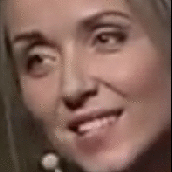
\includegraphics[width=\linewidth]{6178_faceImage_0/cropped_img-12.png}
\end{subfigure}
\begin{subfigure}{0.09\textwidth}
  \centering
  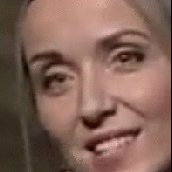
\includegraphics[width=\linewidth]{6178_faceImage_0/cropped_img-13.png}
\end{subfigure}
\begin{subfigure}{0.09\textwidth}
  \centering
  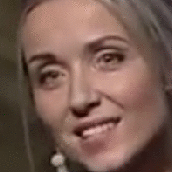
\includegraphics[width=\linewidth]{6178_faceImage_0/cropped_img-14.png}
\end{subfigure}
\begin{subfigure}{0.09\textwidth}
  \centering
  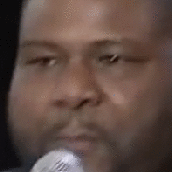
\includegraphics[width=\linewidth]{6178_faceImage_0/cropped_img-15.png}
\end{subfigure}
\begin{subfigure}{0.09\textwidth}
  \centering
  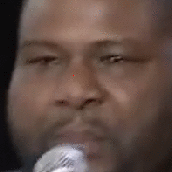
\includegraphics[width=\linewidth]{6178_faceImage_0/cropped_img-16.png}
\end{subfigure}
\begin{subfigure}{0.09\textwidth}
  \centering
  
\includegraphics[width=\linewidth]{6178_faceImage_0/cropped_img-17.png}
\end{subfigure}
\begin{subfigure}{0.09\textwidth}
  \centering
  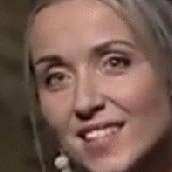
\includegraphics[width=\linewidth]{6178_faceImage_0/cropped_img-18.png}
\end{subfigure}
\begin{subfigure}{0.09\textwidth}
  \centering
  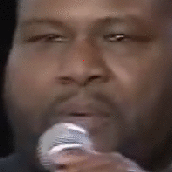
\includegraphics[width=\linewidth]{6178_faceImage_0/cropped_img-19.png}
\end{subfigure}
}
\parbox{\textwidth}{
\begin{subfigure}{0.09\textwidth}
  \centering
  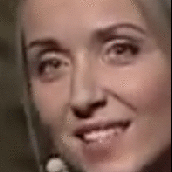
\includegraphics[width=\linewidth]{6178_faceImage_0/cropped_img-20.png}
\end{subfigure}
\begin{subfigure}{0.09\textwidth}
  \centering
  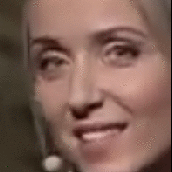
\includegraphics[width=\linewidth]{6178_faceImage_0/cropped_img-21.png}
\end{subfigure}
\begin{subfigure}{0.09\textwidth}
  \centering
  
\includegraphics[width=\linewidth]{6178_faceImage_0/cropped_img-22.png}
\end{subfigure}
\begin{subfigure}{0.09\textwidth}
  \centering
  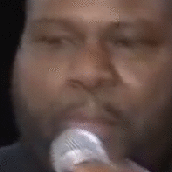
\includegraphics[width=\linewidth]{6178_faceImage_0/cropped_img-23.png}
\end{subfigure}
\begin{subfigure}{0.09\textwidth}
  \centering
  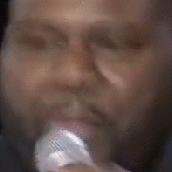
\includegraphics[width=\linewidth]{6178_faceImage_0/cropped_img-24.png}
\end{subfigure}
\begin{subfigure}{0.09\textwidth}
  \centering
  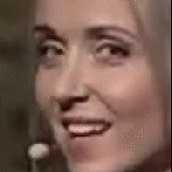
\includegraphics[width=\linewidth]{6178_faceImage_0/cropped_img-25.png}
\end{subfigure}
\begin{subfigure}{0.09\textwidth}
  \centering
  
\includegraphics[width=\linewidth]{6178_faceImage_0/cropped_img-26.png}
\end{subfigure}
\begin{subfigure}{0.09\textwidth}
  \centering
  
\includegraphics[width=\linewidth]{6178_faceImage_0/cropped_img-27.png}
\end{subfigure}
\begin{subfigure}{0.09\textwidth}
  \centering
  
\includegraphics[width=\linewidth]{6178_faceImage_0/cropped_img-28.png}
\end{subfigure}
\begin{subfigure}{0.09\textwidth}
  \centering
  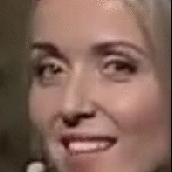
\includegraphics[width=\linewidth]{6178_faceImage_0/cropped_img-29.png}
\end{subfigure}
}
\parbox{\textwidth}{
\begin{subfigure}{0.09\textwidth}
  \centering
  
\includegraphics[width=\linewidth]{6178_faceImage_0/cropped_img-30.png}
\end{subfigure}
\begin{subfigure}{0.09\textwidth}
  \centering
  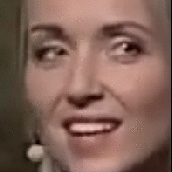
\includegraphics[width=\linewidth]{6178_faceImage_0/cropped_img-31.png}
\end{subfigure}
\begin{subfigure}{0.09\textwidth}
  \centering
  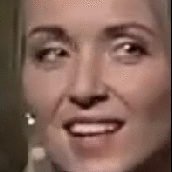
\includegraphics[width=\linewidth]{6178_faceImage_0/cropped_img-32.png}
\end{subfigure}
\begin{subfigure}{0.09\textwidth}
  \centering
  
\includegraphics[width=\linewidth]{6178_faceImage_0/cropped_img-33.png}
\end{subfigure}
\begin{subfigure}{0.09\textwidth}
  \centering
  
\includegraphics[width=\linewidth]{6178_faceImage_0/cropped_img-34.png}
\end{subfigure}
\begin{subfigure}{0.09\textwidth}
  \centering
  
\includegraphics[width=\linewidth]{6178_faceImage_0/cropped_img-35.png}
\end{subfigure}
\begin{subfigure}{0.09\textwidth}
  \centering
  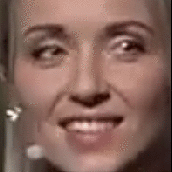
\includegraphics[width=\linewidth]{6178_faceImage_0/cropped_img-36.png}
\end{subfigure}
\begin{subfigure}{0.09\textwidth}
  \centering
  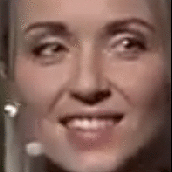
\includegraphics[width=\linewidth]{6178_faceImage_0/cropped_img-37.png}
\end{subfigure}
}
\caption{Sample \texttt{6178} is labeled as a negative (\emph{not speaking}) sample by the automatic transformation from LRS3 to VVAD dataset. On the human accuracy level test 100\% of the subjects classified the sample as positive (\emph{speaking}) sample. Beat boxing is not considered speech in the LRS3 dataset, which causes the wrong label.}
\label{fig:6178}
\end{figure}


\begin{figure}
\centering
\parbox{\textwidth}{
\begin{subfigure}{0.09\textwidth}
  \centering
  \includegraphics[width=\linewidth]{31366_faceImage_1/cropped_img-0.png}
\end{subfigure}
\begin{subfigure}{0.09\textwidth}
  \centering
  \includegraphics[width=\linewidth]{31366_faceImage_1/cropped_img-1.png}
\end{subfigure}
\begin{subfigure}{0.09\textwidth}
  \centering
  \includegraphics[width=\linewidth]{31366_faceImage_1/cropped_img-2.png}
\end{subfigure}
\begin{subfigure}{0.09\textwidth}
  \centering
  \includegraphics[width=\linewidth]{31366_faceImage_1/cropped_img-3.png}
\end{subfigure}
\begin{subfigure}{0.09\textwidth}
  \centering
  
\includegraphics[width=\linewidth]{31366_faceImage_1/cropped_img-4.png}
\end{subfigure}
\begin{subfigure}{0.09\textwidth}
  \centering
  \includegraphics[width=\linewidth]{31366_faceImage_1/cropped_img-5.png}
\end{subfigure}
\begin{subfigure}{0.09\textwidth}
  \centering
  
\includegraphics[width=\linewidth]{31366_faceImage_1/cropped_img-6.png}
\end{subfigure}
\begin{subfigure}{0.09\textwidth}
  \centering
  
\includegraphics[width=\linewidth]{31366_faceImage_1/cropped_img-7.png}
\end{subfigure}
\begin{subfigure}{0.09\textwidth}
  \centering
  
\includegraphics[width=\linewidth]{31366_faceImage_1/cropped_img-8.png}
\end{subfigure}
\begin{subfigure}{0.09\textwidth}
  \centering
  
\includegraphics[width=\linewidth]{31366_faceImage_1/cropped_img-9.png}
\end{subfigure}
}
\parbox{\textwidth}{
\begin{subfigure}{0.09\textwidth}
  \centering
  
\includegraphics[width=\linewidth]{31366_faceImage_1/cropped_img-10.png}
\end{subfigure}
\begin{subfigure}{0.09\textwidth}
  \centering
  \includegraphics[width=\linewidth]{31366_faceImage_1/cropped_img-11.png}
\end{subfigure}
\begin{subfigure}{0.09\textwidth}
  \centering
  \includegraphics[width=\linewidth]{31366_faceImage_1/cropped_img-12.png}
\end{subfigure}
\begin{subfigure}{0.09\textwidth}
  \centering
  \includegraphics[width=\linewidth]{31366_faceImage_1/cropped_img-13.png}
\end{subfigure}
\begin{subfigure}{0.09\textwidth}
  \centering
  \includegraphics[width=\linewidth]{31366_faceImage_1/cropped_img-14.png}
\end{subfigure}
\begin{subfigure}{0.09\textwidth}
  \centering
  \includegraphics[width=\linewidth]{31366_faceImage_1/cropped_img-15.png}
\end{subfigure}
\begin{subfigure}{0.09\textwidth}
  \centering
  \includegraphics[width=\linewidth]{31366_faceImage_1/cropped_img-16.png}
\end{subfigure}
\begin{subfigure}{0.09\textwidth}
  \centering
  \includegraphics[width=\linewidth]{31366_faceImage_1/cropped_img-17.png}
\end{subfigure}
\begin{subfigure}{0.09\textwidth}
  \centering
  \includegraphics[width=\linewidth]{31366_faceImage_1/cropped_img-18.png}
\end{subfigure}
\begin{subfigure}{0.09\textwidth}
  \centering
  \includegraphics[width=\linewidth]{31366_faceImage_1/cropped_img-19.png}
\end{subfigure}
}
\parbox{\textwidth}{
\begin{subfigure}{0.09\textwidth}
  \centering
  \includegraphics[width=\linewidth]{31366_faceImage_1/cropped_img-20.png}
\end{subfigure}
\begin{subfigure}{0.09\textwidth}
  \centering
  \includegraphics[width=\linewidth]{31366_faceImage_1/cropped_img-21.png}
\end{subfigure}
\begin{subfigure}{0.09\textwidth}
  \centering
  \includegraphics[width=\linewidth]{31366_faceImage_1/cropped_img-22.png}
\end{subfigure}
\begin{subfigure}{0.09\textwidth}
  \centering
  \includegraphics[width=\linewidth]{31366_faceImage_1/cropped_img-23.png}
\end{subfigure}
\begin{subfigure}{0.09\textwidth}
  \centering
  \includegraphics[width=\linewidth]{31366_faceImage_1/cropped_img-24.png}
\end{subfigure}
\begin{subfigure}{0.09\textwidth}
  \centering
  \includegraphics[width=\linewidth]{31366_faceImage_1/cropped_img-25.png}
\end{subfigure}
\begin{subfigure}{0.09\textwidth}
  \centering
  \includegraphics[width=\linewidth]{31366_faceImage_1/cropped_img-26.png}
\end{subfigure}
\begin{subfigure}{0.09\textwidth}
  \centering
  \includegraphics[width=\linewidth]{31366_faceImage_1/cropped_img-27.png}
\end{subfigure}
\begin{subfigure}{0.09\textwidth}
  \centering
  \includegraphics[width=\linewidth]{31366_faceImage_1/cropped_img-28.png}
\end{subfigure}
\begin{subfigure}{0.09\textwidth}
  \centering
  \includegraphics[width=\linewidth]{31366_faceImage_1/cropped_img-29.png}
\end{subfigure}
}
\parbox{\textwidth}{
\begin{subfigure}{0.09\textwidth}
  \centering
  \includegraphics[width=\linewidth]{31366_faceImage_1/cropped_img-30.png}
\end{subfigure}
\begin{subfigure}{0.09\textwidth}
  \centering
  \includegraphics[width=\linewidth]{31366_faceImage_1/cropped_img-31.png}
\end{subfigure}
\begin{subfigure}{0.09\textwidth}
  \centering
  \includegraphics[width=\linewidth]{31366_faceImage_1/cropped_img-32.png}
\end{subfigure}
\begin{subfigure}{0.09\textwidth}
  \centering
  \includegraphics[width=\linewidth]{31366_faceImage_1/cropped_img-33.png}
\end{subfigure}
\begin{subfigure}{0.09\textwidth}
  \centering
  \includegraphics[width=\linewidth]{31366_faceImage_1/cropped_img-34.png}
\end{subfigure}
\begin{subfigure}{0.09\textwidth}
  \centering
  \includegraphics[width=\linewidth]{31366_faceImage_1/cropped_img-35.png}
\end{subfigure}
\begin{subfigure}{0.09\textwidth}
  \centering
  \includegraphics[width=\linewidth]{31366_faceImage_1/cropped_img-36.png}
\end{subfigure}
\begin{subfigure}{0.09\textwidth}
  \centering
  \includegraphics[width=\linewidth]{31366_faceImage_1/cropped_img-37.png}
\end{subfigure}
}
\caption{Sample \texttt{31366} is labeled as a positive (\emph{speaking}) sample by the automatic transformation from LRS3 to VVAD dataset. On the human accuracy level test 100\% of the subjects classified the sample as negative (\emph{not speaking}) sample. The fast movement of the head while producing only a small movement of the lips causes the wrong label.}
\label{fig:31366}
\end{figure}

\section{End-to-End Learning}
As described in Section \ref{ssec:EndToEndLearning} the models trained on images of faces or lips perform quite well on the validation set.
Here accuracies over 90\% could be reached.
The test described earlier reaches a \emph{test accuracy} of 92\% 
for the model trained on faces.
This model has a MAE of $0.08$. 
The classifications of this can be seen in Figure \ref{fig:testFaceImages}.
The first 100 samples are negative samples while the last 100 samples are positive samples and the arrows show the probability, given by the model, that this sample belongs to the positive class.
The red dashed line is the decision boundary on which the model decides its classifications. 
This visualizeses how certain the model is with its predictions.

The smaller model which was only trained on images of the lips reaches a \emph{test accuracy} of 92\% with a MAE of $0.09$.
The classifications on the test set made by this model are depicted in Figure \ref{fig:testLipImages}.
Similar to the performances in the validation set the performances in the test set are very close to each other.
The bigger model adds only a very small improvement to the \emph{test accuracy}

\begin{figure}
  \centering
  \includegraphics[width=.75\textwidth]{testFaceImages.png}
  \caption{Visualization of the classifications on the test set for the model which was trained on images of faces.}
  \label{fig:testFaceImages}
\end{figure}

\begin{figure}
  \centering
  \includegraphics[width=.75\textwidth]{testLipImages.png}
  \caption{Visualization of the classifications on the test set for the model which was trained on images of lips.}
  \label{fig:testLipImages}
\end{figure}

The performance on the wrong labeled samples described in Section \ref{sec:wrongLabels} is shown in Figure \ref{fig:testWrongFaceImages} - \ref{fig:testWrongLipImages}.
Here it can be seen that the model performs exactly the same as the human subjects in the human accuracy level test.

\begin{figure}
  \centering
  \includegraphics[width=.75\textwidth]{testWrongFaceImages.png}
  \caption{Visualization of the classifications on wrong labeled samples in the test set for the model which was trained on images of faces.}
  \label{fig:testWrongFaceImages}
\end{figure}

\begin{figure}
  \centering
  \includegraphics[width=.75\textwidth]{testWrongLipImages.png}
  \caption{Visualization of the classifications on wrong labeled samples in the test set for the model which was trained on images of lips.}
  \label{fig:testWrongLipImages}
\end{figure}


\section{Learning on Facial Features}
As described in Section \ref{ssec:facialFeaturesLearninig} the models trained on the facial landmarks perform quite well on the validation set.
For the model trained on all 68 facial landmarks the conducted test delivered a \emph{test accuracy} of 89\%
and a MAE of $0.15$. 
This shows that the model also generalizes very well on data it was never in contact with.
Figure \ref{fig:testFaceFeatures} shows the classifications made by the model.


\begin{figure}
  \centering
  \includegraphics[width=.75\textwidth]{testFaceFeatures.png}
  \caption{Visualization of the classifications on the test set for the model which uses all 68 facial landmarks.}
  \label{fig:testFaceFeatures}
\end{figure}

\begin{figure}
  \centering
  \includegraphics[width=.75\textwidth]{testLipFeatures.png}
  \caption{Visualization of the classifications on the test set for the model which uses the 20 facial landmarks corresponding to the lips.}
  \label{fig:testLipFeatures}
\end{figure}

While in the validation set the model trained on the 20 facial landmarks corresponding to the lips performed nearly the same this behavior hold in the test set.
Figure \ref{fig:testLipFeatures} shows the classifications made by the model.
The model reaches a \emph{test accuracy} of 89\% with a MAE of $0.16$.
This shows that the models are performing nearly the same although the model trained on the face features is 1.4 times bigger than the model trained on the lip features.
Although the models trained on the facial features perform nearly as good as the ones using the End-To-End Learning approach Figure \ref{fig:testFaceImages} - \ref{fig:testLipFeatures} visualize very well the fact that the End-To-End models have less uncertainty in their predictions.

The performance on the wrong labeled samples for the models trained on facial features are depicted in Figure \ref{fig:testWrongFaceFeatures} - \ref{fig:testWrongLipFeatures}.
These results show that the model trained only on the facial landmarks of the lips was able to correctly classify sample \texttt{31366} although humans were not able to do so. 
Also sample \texttt{6178} shows a prediction closer to the decision boundary which means the model has a higher uncertainty on this classification.

\begin{figure}
  \centering
  \includegraphics[width=.75\textwidth]{testWrongFaceFeatures.png}
  \caption{Visualization of the classifications on wrong labeled samples in the test set for the model which uses all 68 facial landmarks.}
  \label{fig:testWrongFaceFeatures}
\end{figure}

\begin{figure}
  \centering
  \includegraphics[width=.75\textwidth]{testWrongLipFeatures.png}
  \caption{Visualization of the classifications on wrong labeled samples in the test set for the model which uses the 20 facial landmarks corresponding to the lips.}
  \label{fig:testWrongLipFeatures}
\end{figure}


\section{Interpretation}\label{sec:interpretation}
All described models reach a \emph{superhuman performance} not only while validation but also in the test set.
Table \ref{tb:accuracies} shows an overview of the accuracies reached by the different approaches.

\begin{table}[h!]
\centering
\begin{tabular}{|l|c|c|}
\hline
\textbf{Model} & \textbf{Accuracy} & \textbf{MAE} \\
\hline
Face Images & 92\% & 0.08 \\
\hline
Lip Images & 92\% & 0.09 \\
\hline
Face Features &  89\% & 0.15 \\
\hline
Lip Features & 89\% & 0.16 \\
\hline
\end{tabular}
\caption{Overview of the performance of the different models}
\label{tb:accuracies}
\end{table}

This shows that the cognitive skill can be used very reliable to improve various applications in the field of social robotics to make Human-Machine-Interaction more natural.
Additionally it was shown that the assumption that VVAD mostly depends on the lips holds true.
This helps to understand VVAD in more depth and makes it possible to generate smaller models while sustaining high accuracy.
Furthermore it was shown that \emph{Deep Learning} is a very generic approach that can reach very high accuracy but on the downside produces very big models and modern GPUs might reach their limits training such models.
In this aspect, research is required to design techniques that use regularization during training time to allow the model to shrink during training.
Until more robust and clever regularization mechanism are found \emph{feature engineering} is still a valuable task in the world of machine learning to reduce model size and training time.
This is highlighted by the results of the models trained on the facial landmarks that reach nearly as high accuracy as the End-To-End approaches but consume only a fraction of the memory and also the training time could be reduced massively.
Besides that feature engineering brings the advantage that the human designer of the learning algorithm can very precisely define what features will be used to learn which gives more comprehensibility to the designed algorithm.
But it also limits the model to the assumptions made by the human designer.
This can be shown in the comparison of the End-To-End approach and the feature engineered approach using the facial landmarks.
The latter shows more instability in the learning as seen in Figure \ref{fig:FaceFeaturesHistory} and a higher uncertainty in the predictions shown in Figure \ref{fig:testFaceFeatures} and a higher MAE for this approach.
